\section{Architettura}

%%%%%%%%%%%%%%%%%%%%%%%%%%%%%%%%%%%%%%%%%%%%%%%%%%%%%%%%%%%%%%%%%%%%%%%%%%%%%%%%%%
\subsection{Introduzione all’architettura}
    \subsubsection{Scopo e obbiettivi}
    La presente sezione ha lo scopo di fornire una visione d’insieme dell’architettura del sistema, evidenziandone i principi guida e le scelte progettuali che ne hanno determinato la struttura. In particolare, si intende:
    \begin{itemize}
        \item Definire il contesto in cui opera il sistema, evidenziando i requisiti funzionali e non funzionali che hanno condotto alla scelta di una specifica architettura.
        \item Orientare i lettori (sviluppatori, progettisti e stakeholder) verso una comprensione chiara delle componenti principali e delle interazioni che caratterizzano il sistema.
        \item Porre le basi per la discussione delle scelte di design, evidenziando come queste possano rispondere alle esigenze di scalabilità, sicurezza, manutenibilità e performance.
        \item Descrivere le motivazioni alla base delle scelte tecnologiche e dei modelli architetturali adottati.
    \end{itemize}



%%%%%%%%%%%%%%%%%%%%%%%%%%%%%%%%%%%%%%%%%%%%%%%%%%%%%%%%%%%%%%%%%%%%%%%%%%%%%%%%%%

\subsection{Architettura del sistema}
La progettazione dell’architettura del sistema ha richiesto un’approfondita analisi delle due principali opzioni architetturali disponibili: \textbf{monolitica} e \textbf{a microservizi}. La scelta dell’architettura è stata guidata da una serie di fattori, tra cui la natura dell’applicazione, il volume di traffico previsto, i costi di sviluppo e manutenzione e la necessità di scalabilità. In questa sezione verranno analizzati nel dettaglio i pro e i contro di entrambe le soluzioni, per poi motivare la decisione finale.
\subsubsection{Architettura monolitica}
Un’architettura monolitica si basa su un’unica codebase che incorpora tutti i componenti dell’applicazione, tra cui l’interfaccia utente, la logica di business e il livello di accesso ai dati. Questo approccio, tradizionalmente adottato nello sviluppo software, è particolarmente indicato per applicazioni di piccola e media complessità, in cui i costi di separazione dei componenti in unità indipendenti non sono giustificati.
\paragraph{Vantaggi}  
\begin{itemize}
    \item \textbf{Semplicità di sviluppo e gestione}: Un’unica codebase permette di mantenere una visione centralizzata del sistema, semplificando lo sviluppo, il testing e il debugging.
    \item \textbf{Minori costi di infrastruttura}: Non è necessario investire in strumenti di orchestrazione, load balancing o gestione della comunicazione tra microservizi.
    \item \textbf{Deployment più semplice}: L’intero sistema viene distribuito come un’unica unità, evitando problemi di coordinamento.
    \item \textbf{Prestazioni migliori per bassi volumi di traffico}: L’assenza di chiamate di rete tra microservizi riduce la latenza.
\end{itemize}
\paragraph{Svantaggi}  
\begin{itemize}
    \item \textbf{Scalabilità limitata}: Non è possibile scalare singole componenti separatamente.
    \item \textbf{Maggiore impatto degli errori}: Un bug in una parte dell’applicazione può compromettere l’intero sistema.
    \item \textbf{Difficoltà nell’adozione di nuove tecnologie}: L’aggiornamento di singole parti è complesso poiché l’intero stack è integrato.
\end{itemize}

\subsubsection{Architettura a microservizi}
L’architettura a microservizi suddivide il sistema in componenti indipendenti, ognuno responsabile di una funzionalità specifica. Ogni microservizio comunica con gli altri attraverso API, permettendo un alto grado di indipendenza e flessibilità nello sviluppo.
\paragraph{Vantaggi}  
\begin{itemize}
    \item \textbf{Scalabilità orizzontale}: Ogni microservizio può essere scalato indipendentemente.
    \item \textbf{Flessibilità nello sviluppo}: Permette l’adozione di tecnologie diverse per ciascun servizio.
    \item \textbf{Maggiore resilienza}: Un errore in un microservizio non compromette l’intero sistema.
    \item \textbf{Facilità di manutenzione}: È possibile distribuire aggiornamenti senza dover ripubblicare l’intera applicazione.
\end{itemize}
\paragraph{Svantaggi}  
\begin{itemize}
    \item \textbf{Maggiore complessità gestionale}: L’orchestrazione dei microservizi richiede strumenti avanzati.
    \item \textbf{Comunicazione tra servizi}: Introduce latenza e potenziali colli di bottiglia.
    \item \textbf{Deployment più complesso}: Coordinare il rilascio di più servizi è più oneroso.
    \item \textbf{Costi di sviluppo più elevati}: La frammentazione del sistema richiede maggiore sforzo di progettazione e testing.
\end{itemize}

\subsubsection{Scelta del monolite esagonale}
Dopo un’analisi approfondita, il team di sviluppo ha deciso di adottare un’\textbf{architettura monolitica esagonale}. Questa scelta è stata motivata dai seguenti fattori:
\begin{enumerate}
    \item \textbf{Basso carico di utenti}: L’applicazione è destinata a un contesto B2B con un numero limitato di utenti concorrenti.
    \item \textbf{Semplicità di gestione}: La manutenzione di un monolite è più diretta rispetto a un sistema distribuito.
    \item \textbf{Riduzione dei costi operativi}: L’assenza di strumenti di orchestrazione riduce significativamente i costi di infrastruttura.
    \item \textbf{Velocità di sviluppo}: Un’unica codebase consente iterazioni rapide senza dipendenze tra servizi separati.
    \item \textbf{Evoluzione graduale verso microservizi}: Adottando un’architettura \textbf{esagonale}, il sistema può essere trasformato gradualmente in microservizi senza riscrivere tutto.
\end{enumerate}

\subsection{Architettura esagonale}
L’\textbf{architettura esagonale}, nota anche come \textit{Ports and Adapters}, è un pattern architetturale l'obiettivo di rendere il software più flessibile, testabile e indipendente dalle tecnologie esterne. Questo approccio enfatizza la separazione tra la logica di business e le interfacce di comunicazione con il mondo esterno.

\subsubsection{Principi fondamentali}
L'architettura esagonale si basa su tre concetti chiave:
\begin{itemize}
    \item \textbf{Isolamento della logica di business}: Il core dell'applicazione è indipendente dai dettagli implementativi esterni.
    \item \textbf{Utilizzo di porte e adattatori}: Le \textit{porte} definiscono le interfacce per la comunicazione tra il core e il mondo esterno, mentre gli \textit{adattatori} implementano queste interfacce per specifiche tecnologie.
    \item \textbf{Sostituibilità delle dipendenze}: È possibile cambiare database, framework web o altre dipendenze senza impattare il core.
\end{itemize}

\subsubsection{Struttura dell’architettura esagonale}
L’architettura esagonale può essere rappresentata con tre livelli principali:
\begin{enumerate}
    \item \textbf{Core (Dominio e Logica di Business)}: Contiene le regole fondamentali dell’applicazione.
    \item \textbf{Porte (Ports)}: Interfacce che definiscono i punti di ingresso e uscita del sistema.
    \item \textbf{Adattatori (Adapters)}: Implementazioni concrete delle porte per database, servizi esterni e UI.
\end{enumerate}
\begin{figure}[H]
    \centering
    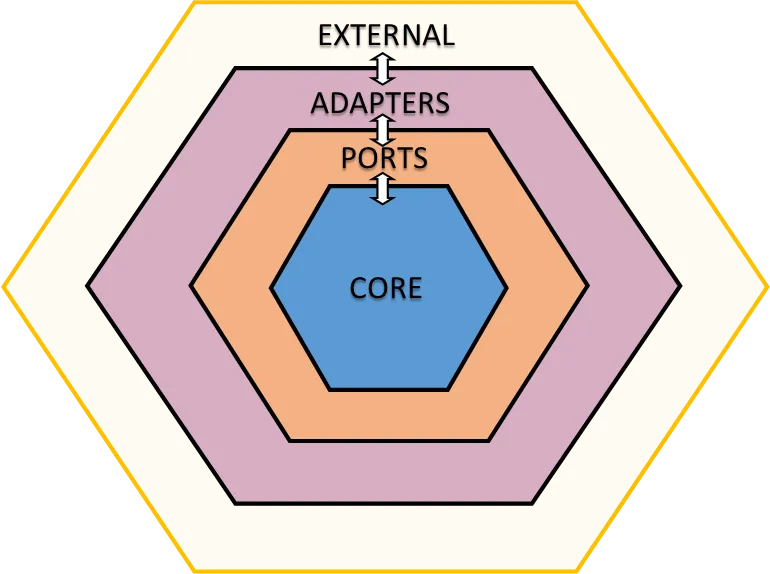
\includegraphics[width=0.7\textwidth]{./img/hexagonal_architecture.png}
    \caption{Schema dell'architettura esagonale}
    \label{fig:hex_arch}
\end{figure}

\subsubsection{Vantaggi dell’architettura esagonale}
Adottare un'architettura esagonale comporta diversi benefici:
\begin{itemize}
    \item \textbf{Maggiore manutenibilità}: Il codice è modulare e separato.
    \item \textbf{Facilità di test}: Il core dell’applicazione può essere testato isolatamente.
    \item \textbf{Indipendenza dalle tecnologie}: Cambiare framework o database ha un impatto minimo.
    \item \textbf{Flessibilità evolutiva}: Permette di trasformare gradualmente il monolite in microservizi.
\end{itemize}

\subsubsection{Conclusione}
L’architettura esagonale garantisce modularità e sostenibilità del sistema nel lungo termine, permettendo di scalare senza impattare la stabilità complessiva dell’applicazione.







%%%%%%%%%%%%%%%%%%%%%%%%%%%%%%%%%%%%%%%%%%%%%%%%%%%%%%%%%%%%%%%%%%%%%%%%%%%%%%%%%%

\subsection{Moduli}
%%%%%%%%%%%%%%%%%%%%%%%%%%%%%%%%%%%%%%%%%%%%%%%%%%%%%%%%%%%%%%%%%%%%%%%%%%%%%%%%%%
\subsection{Tecnologie}
%%%%%%%%%%%%%%%%%%%%%%%%%%%%%%%%%%%%%%%%%%%%%%%%%%%%%%%%%%%%%%%%%%%%%%%%%%%%%%%%%%
\subsubsection{OpenAI API}
%%%%%%%%%%%%%%%%%%%%%%%%%%%%%%%%%%%%%%%%%%%%%%%%%%%%%%%%%%%%%%%%%%%%%%%%%%%%%%%%%%

